\subsection{Relations among features}
So far, we only really looked into features separately. This section will now focus on showing how multiple features are related. We will only consider relating TWO features, but the techniques are also applicable to more.

\subsubsection*{Scatter plots}

As a first step to see whether a relation exists, first plot the two features. Examples for typical resulting \textbf{correlations}\sidenote{Correlation} are shown in \ref{fig:2_correlation}.

\begin{figure}[H]
  \begin{subfigure}{0.3\textwidth}
    \centering
    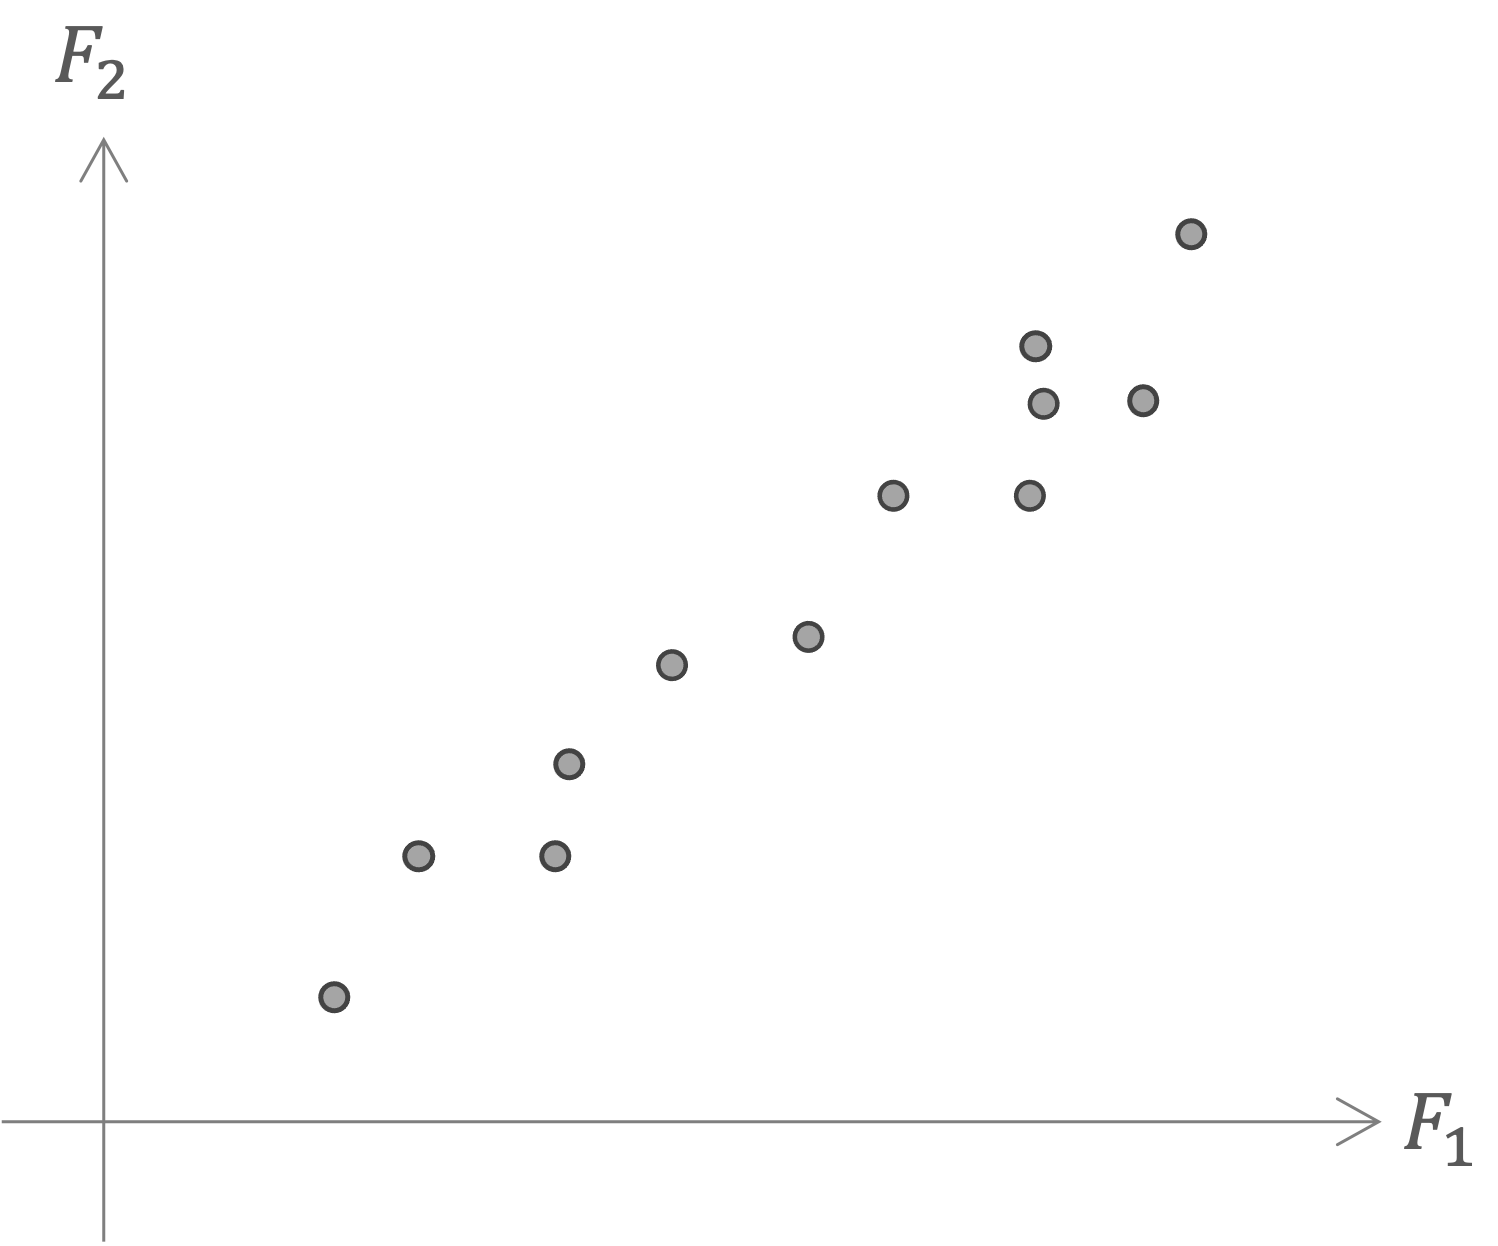
\includegraphics[width=0.8\textwidth]{assets/visualization_and_extraction/feature_relation/scatter_pos_cor.png}
    \subcaption{Positive correlation}
  \end{subfigure}\hspace*{0.025\textwidth}
  \begin{subfigure}{0.3\textwidth}
    \centering
    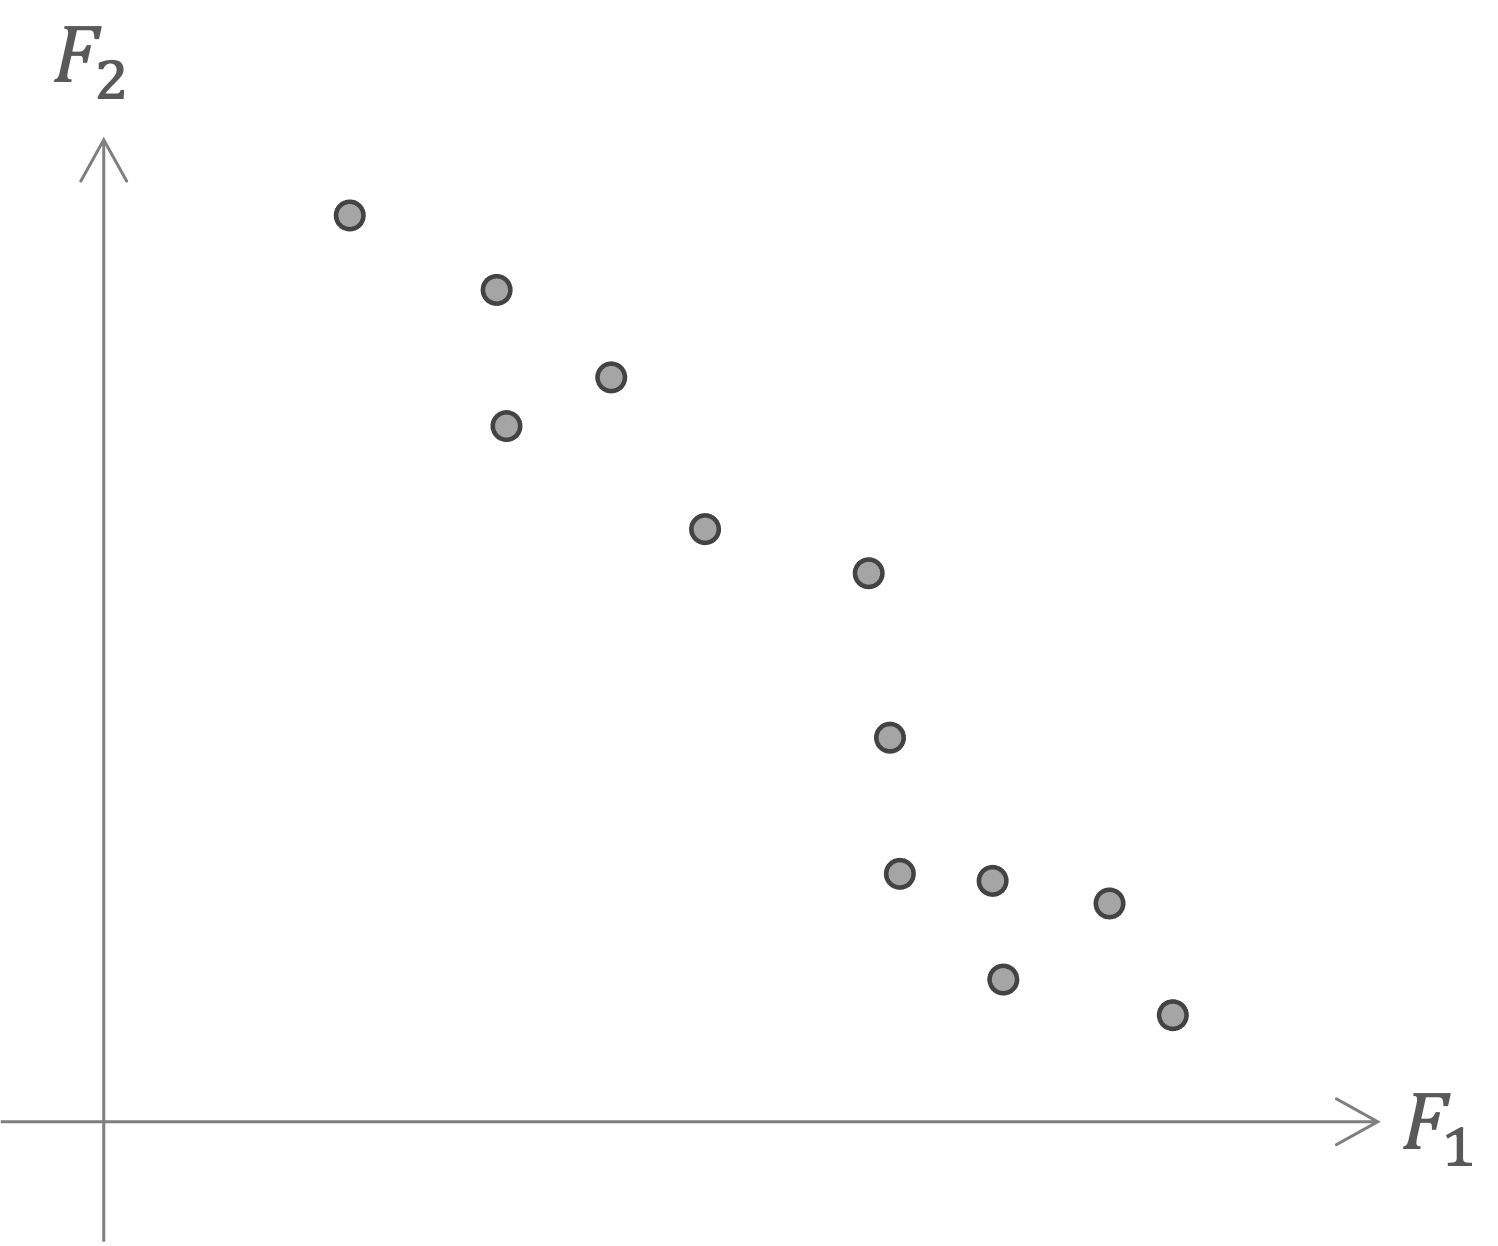
\includegraphics[width=0.8\textwidth]{assets/visualization_and_extraction/feature_relation/scatter_neg_cor.png}
    \subcaption{Negative correlation}
  \end{subfigure}\hspace*{0.025\textwidth}
  \begin{subfigure}{0.3\textwidth}
    \centering
    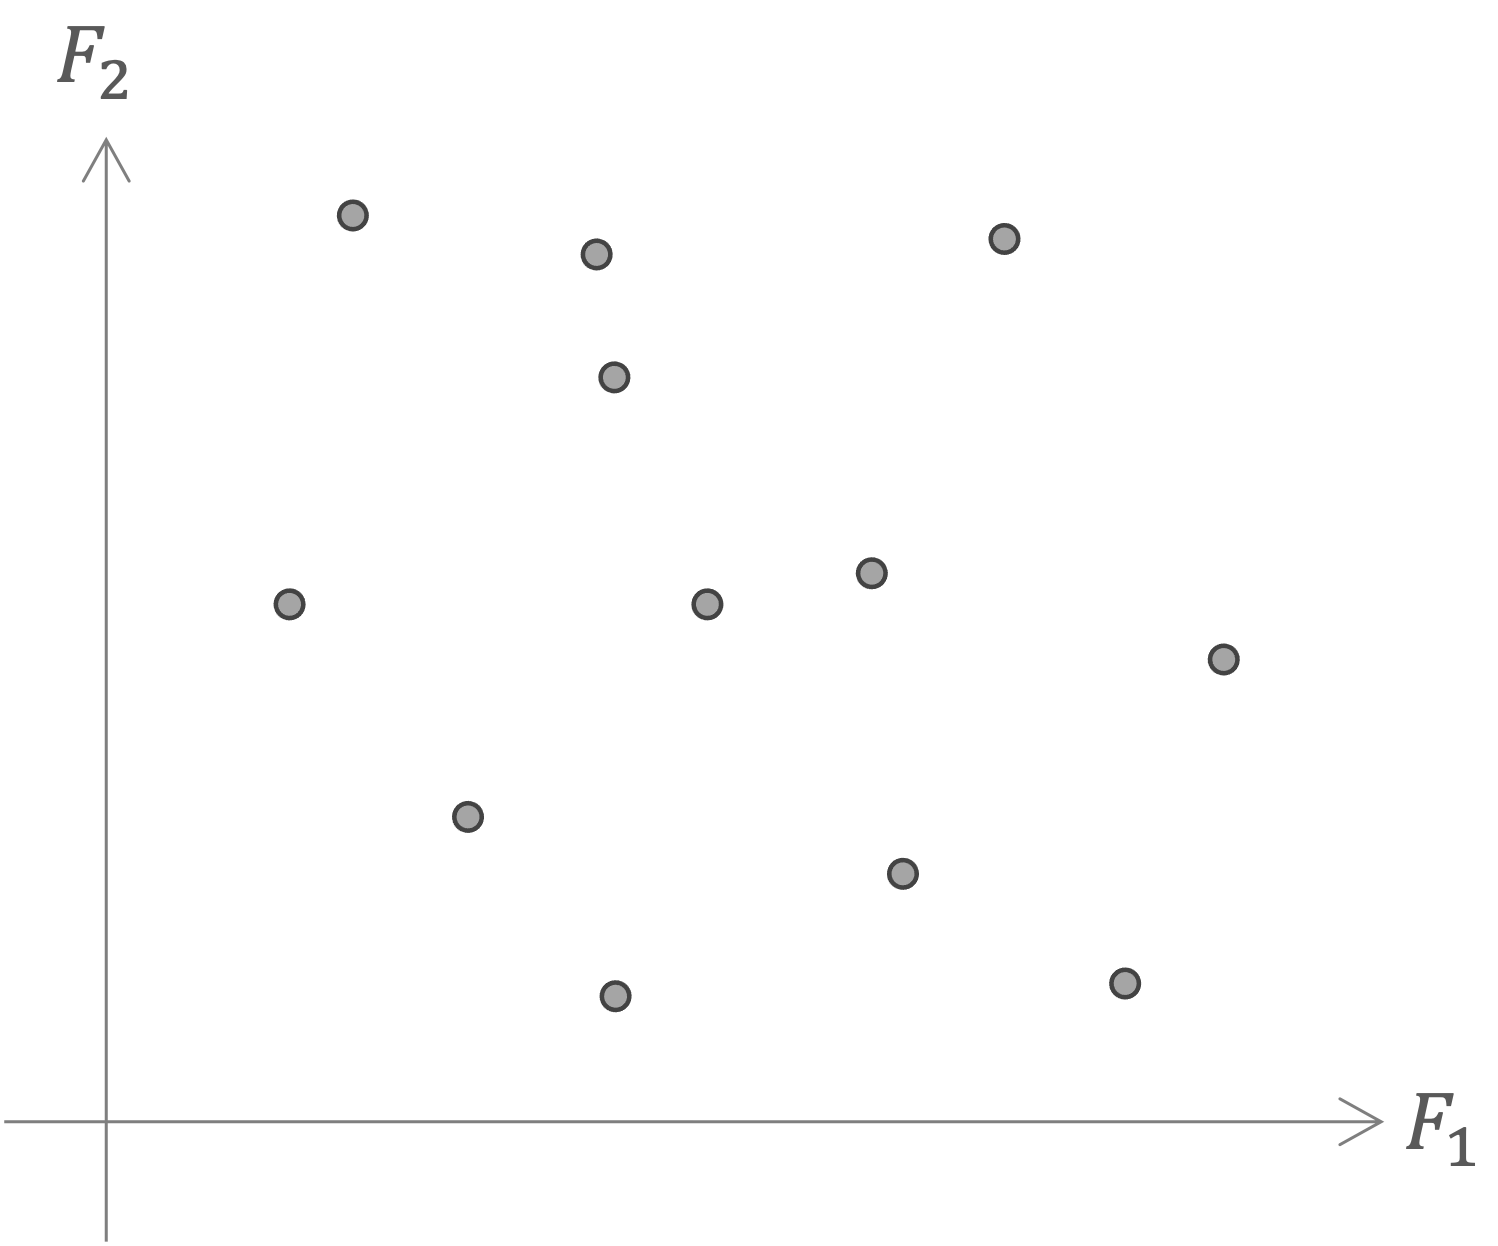
\includegraphics[width=0.8\textwidth]{assets/visualization_and_extraction/feature_relation/scatter_not_cor.png}
    \subcaption{No correlation}
  \end{subfigure}
  \caption{Scatter plots visualizing correlations}
  \label{fig:2_correlation}
\end{figure}

\begin{note}As an example for detecting correlations, we have a data set about basketball players with different features. The raw data will not be included here. Instead, we will directly \end{note}look at all correlations of the features simultaneously. This is visualized using a \textbf{scatter plot matrix} (SPLOM)\sidenote{SPLOM} as in \ref{fig:2_splom}.

\begin{figure}[h]
  \centering
  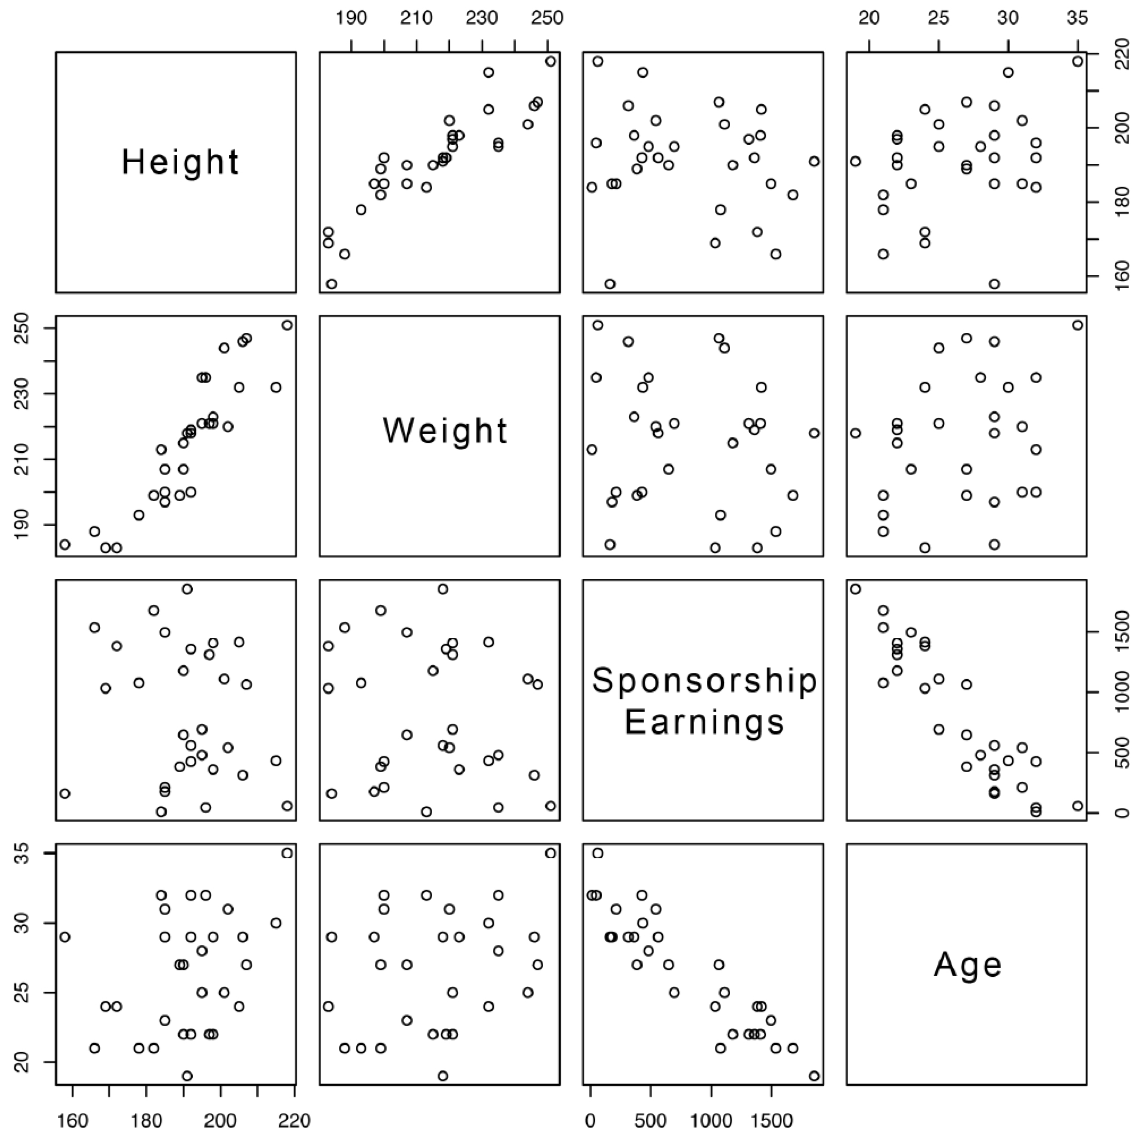
\includegraphics[width=0.6\textwidth]{assets/visualization_and_extraction/feature_relation/splom.png}
  \caption{Scatter plot matrix for four features}
  \label{fig:2_splom}
\end{figure}

Interesting to see in such a SPLOM is the mirror axis in opposite tiles of the matrix which is an absolutely linear line (so absolute correlation, or identity, as would be displayed if a feature would be displayed on a scatter plot compared to itself). This mirroring doesn't change the nature of a correlation. If feature A is positively correlated to feature B, the same goes in the other direction (equivalently for negative correlation).

\subsubsection*{Collection of bar plots}

Another way to display relations is via a collection of small multiple \textbf{bar plots}\sidenote{Collection of small multiple bar plots}. Consider the plots in \ref{fig:2_barplot}

\begin{figure}[h]
  \centering
  \begin{subfigure}{0.85\textwidth}
    \centering
    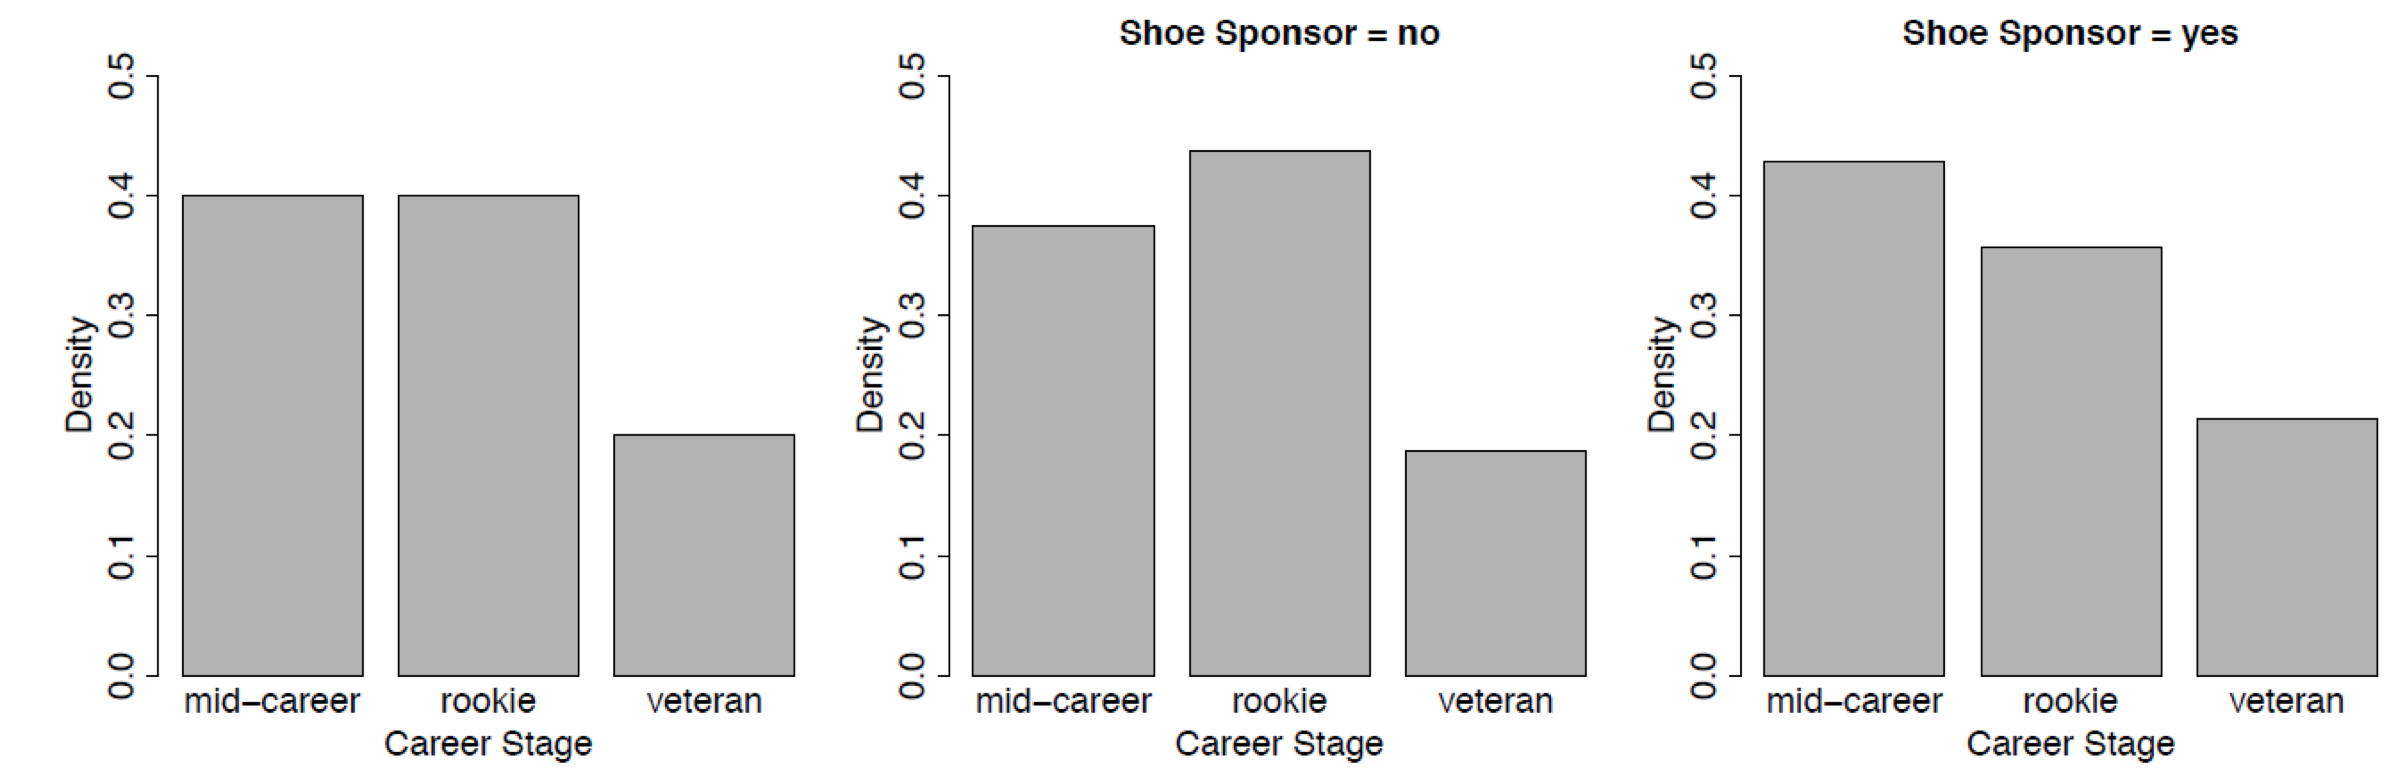
\includegraphics[width=\textwidth]{assets/visualization_and_extraction/feature_relation/bar_no.png}
    \subcaption{Career stage: No relation to shoe sponsor}
  \end{subfigure}
  
  \vspace*{0.2cm}

  \begin{subfigure}{0.8\textwidth}
    \centering
    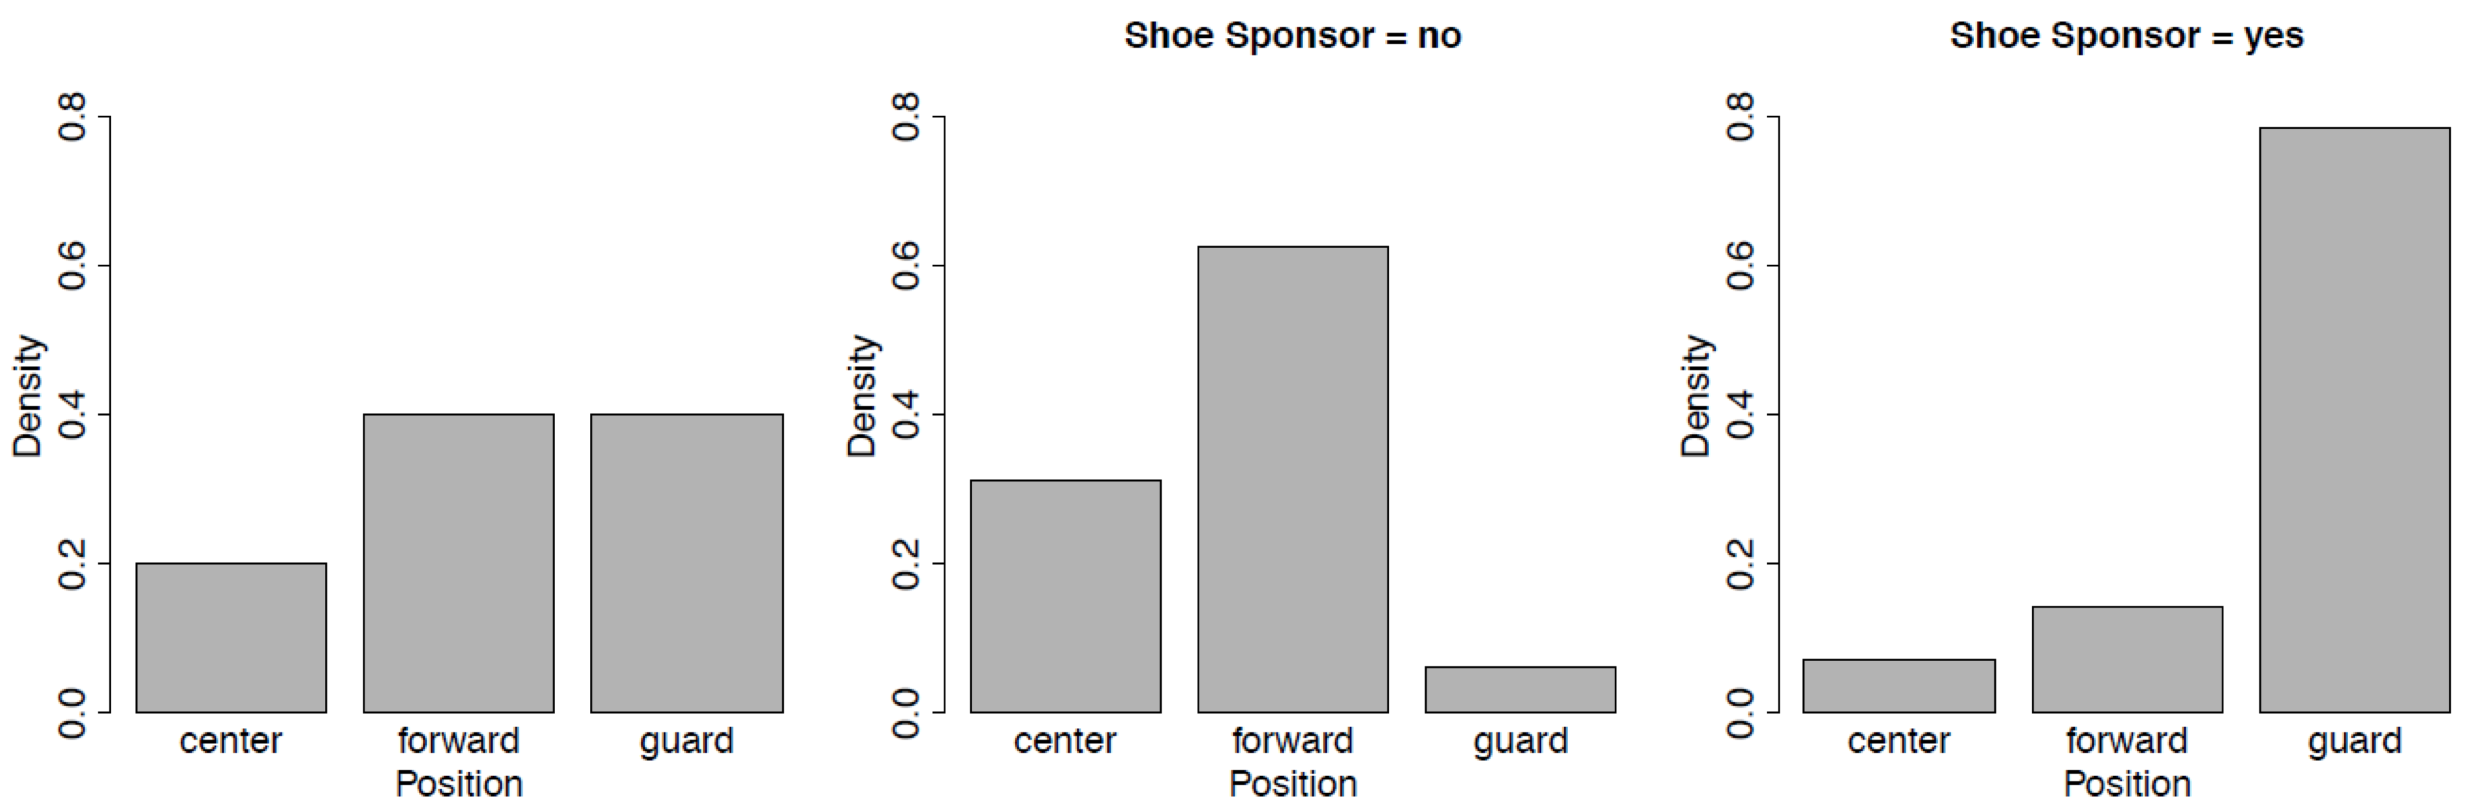
\includegraphics[width=\textwidth]{assets/visualization_and_extraction/feature_relation/bar_strong.png}
    \subcaption{Position: Strong relation to show sponsor}
  \end{subfigure}
  \caption{Collection of (conditioned) bar plots \textcolor{gray}{\footnotesize (Conditioned on shoe sponsor)}}
  \label{fig:2_barplot}
\end{figure}

No relation is implied when the differently conditioned and non-conditioned bar plots don't show any significant difference, as for the example of career stages. On the other hand, a relation can be seen when the bar plots show specific differences. \begin{note}For example in the position case it can be seen that "guards" are more likely to have a shoe sponsor.\end{note}

The difference and implied relation can be further highlighted by using \textbf{stacked bar plots}\sidenote{Stacked bar plots} that show the conditioned percentage, as can be seen in \ref{fig:2_barplot_stack}.

\begin{figure}[H]
  \centering
  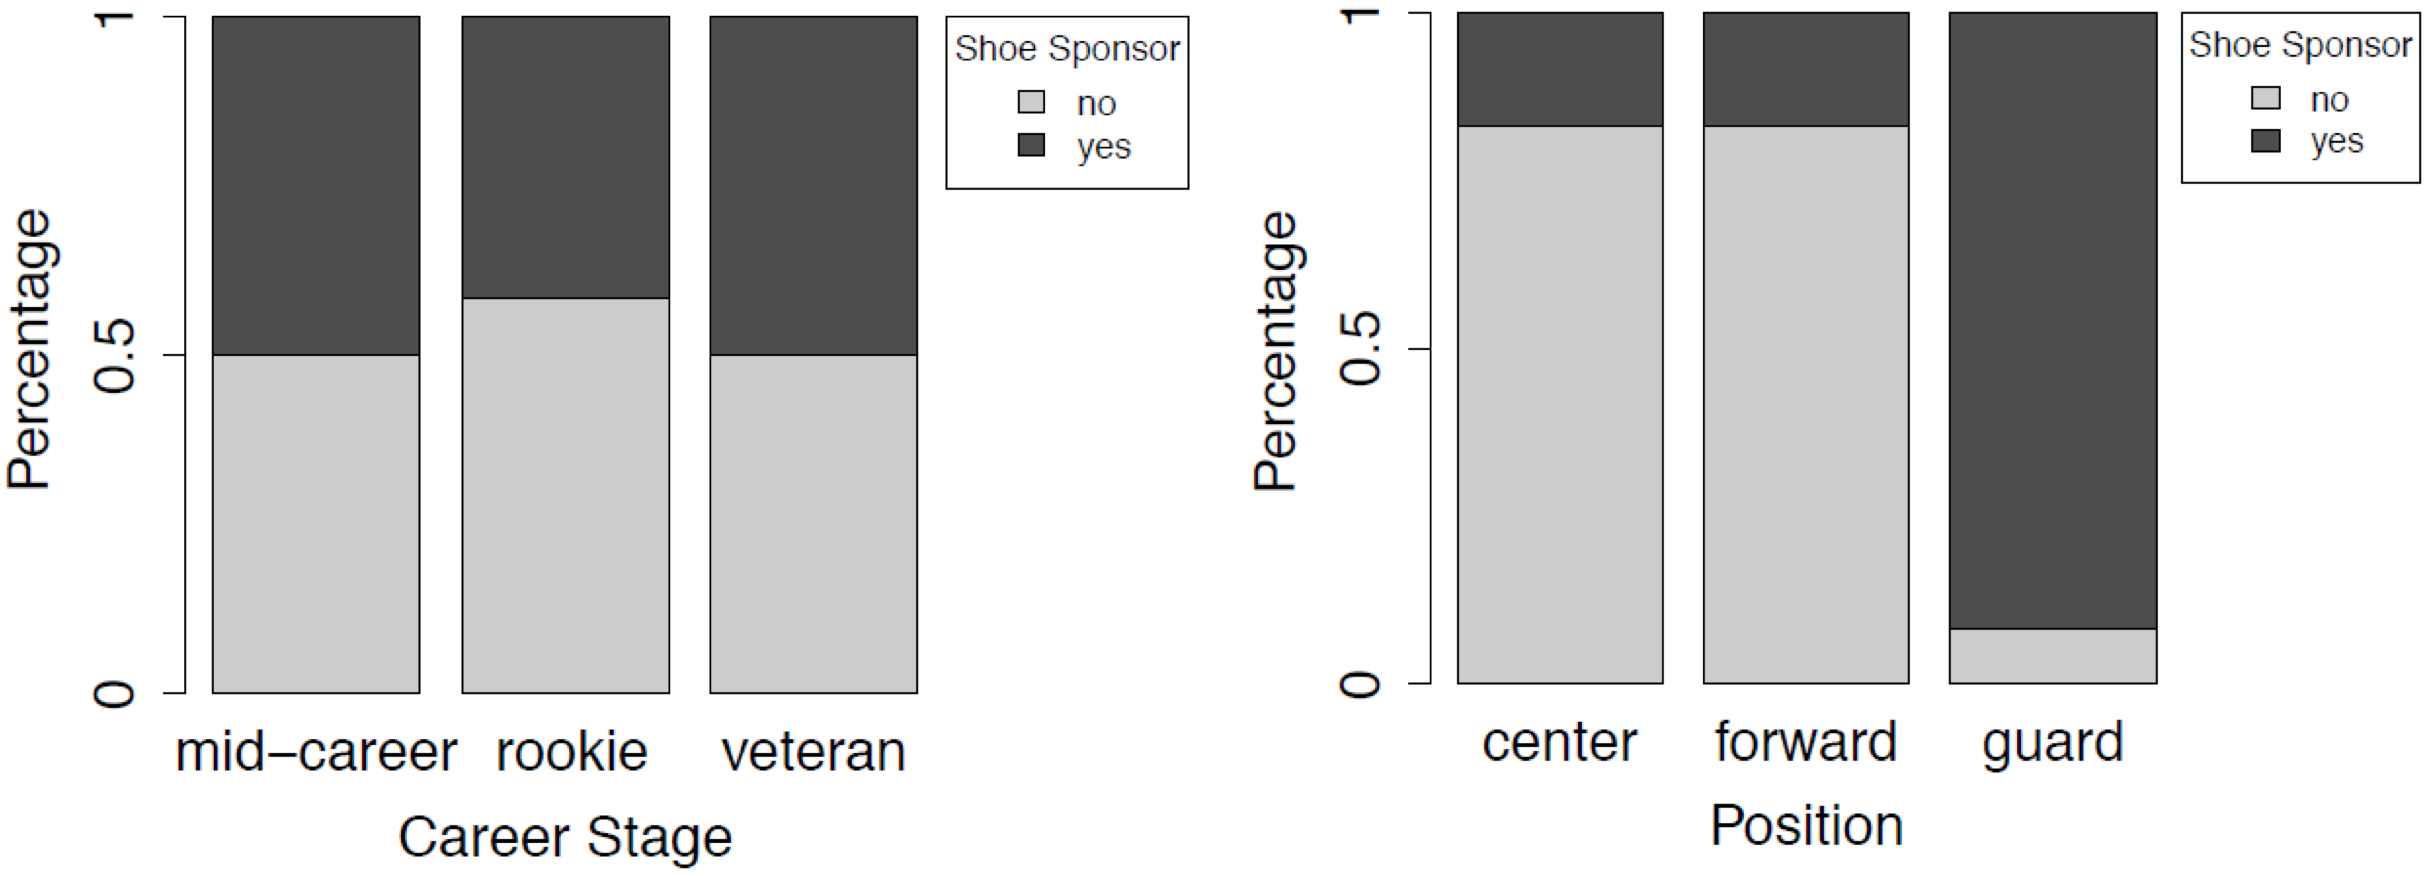
\includegraphics[width=0.75\textwidth]{assets/visualization_and_extraction/feature_relation/bar_stacked.png}
  \caption{Stacked bar plots \textcolor{gray}{\footnotesize (for both career and position conditioned on shoe sponsor)}}
  \label{fig:2_barplot_stack}
\end{figure}

\subsection*{Collection of histograms and box plots}

In the case of continuous variables, instead of bar plots, we can use a collection of small multiple \textbf{histograms}\sidenote{Collection of small multiple histograms}, as displayed in \ref{fig:2_histoplot}.

\begin{figure}[H]
  \centering
  \begin{subfigure}{0.8\textwidth}
    \centering
    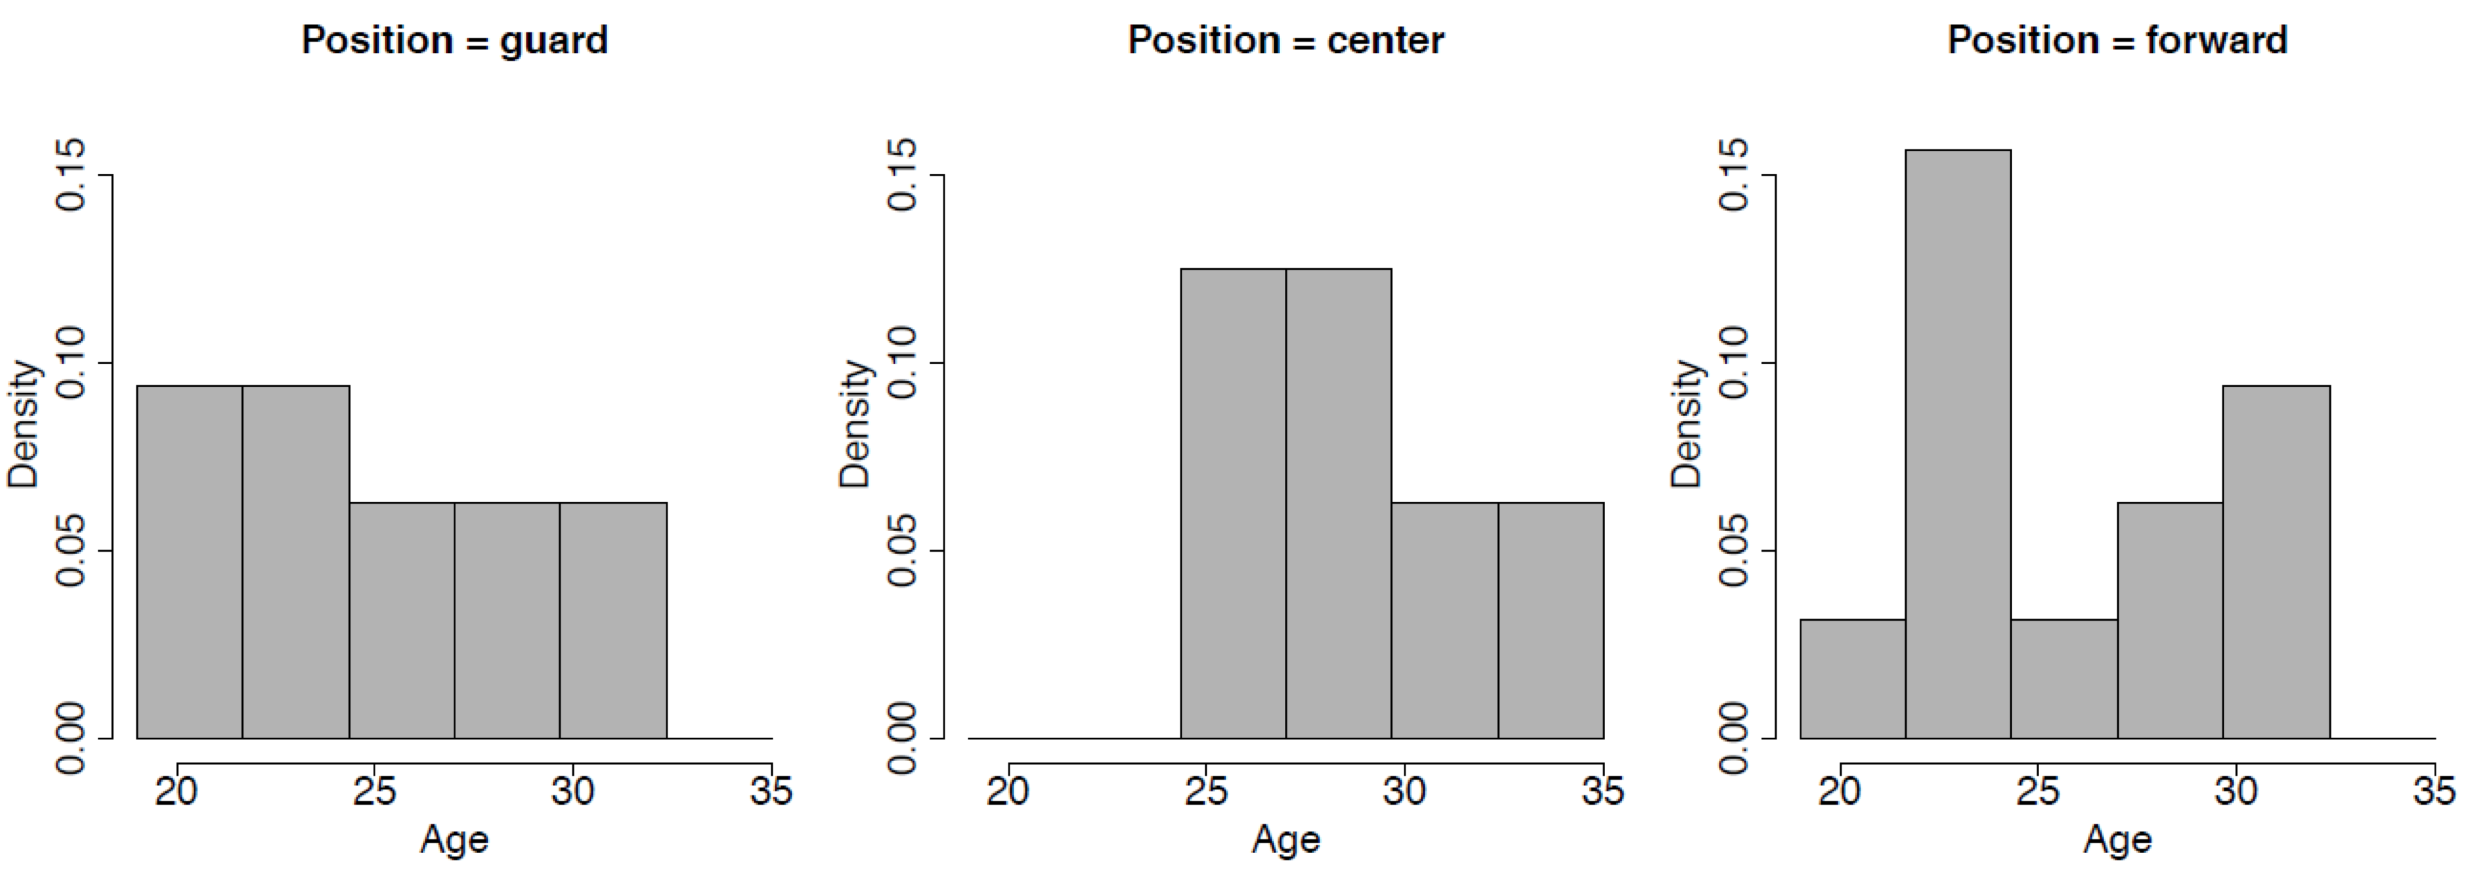
\includegraphics[width=\textwidth]{assets/visualization_and_extraction/feature_relation/histo_no.png}
    \subcaption{Age \textcolor{gray}{\footnotesize (6 bins)}: No strong relation to position}
  \end{subfigure}
  
  \vspace*{0.2cm}

  \begin{subfigure}{0.8\textwidth}
    \centering
    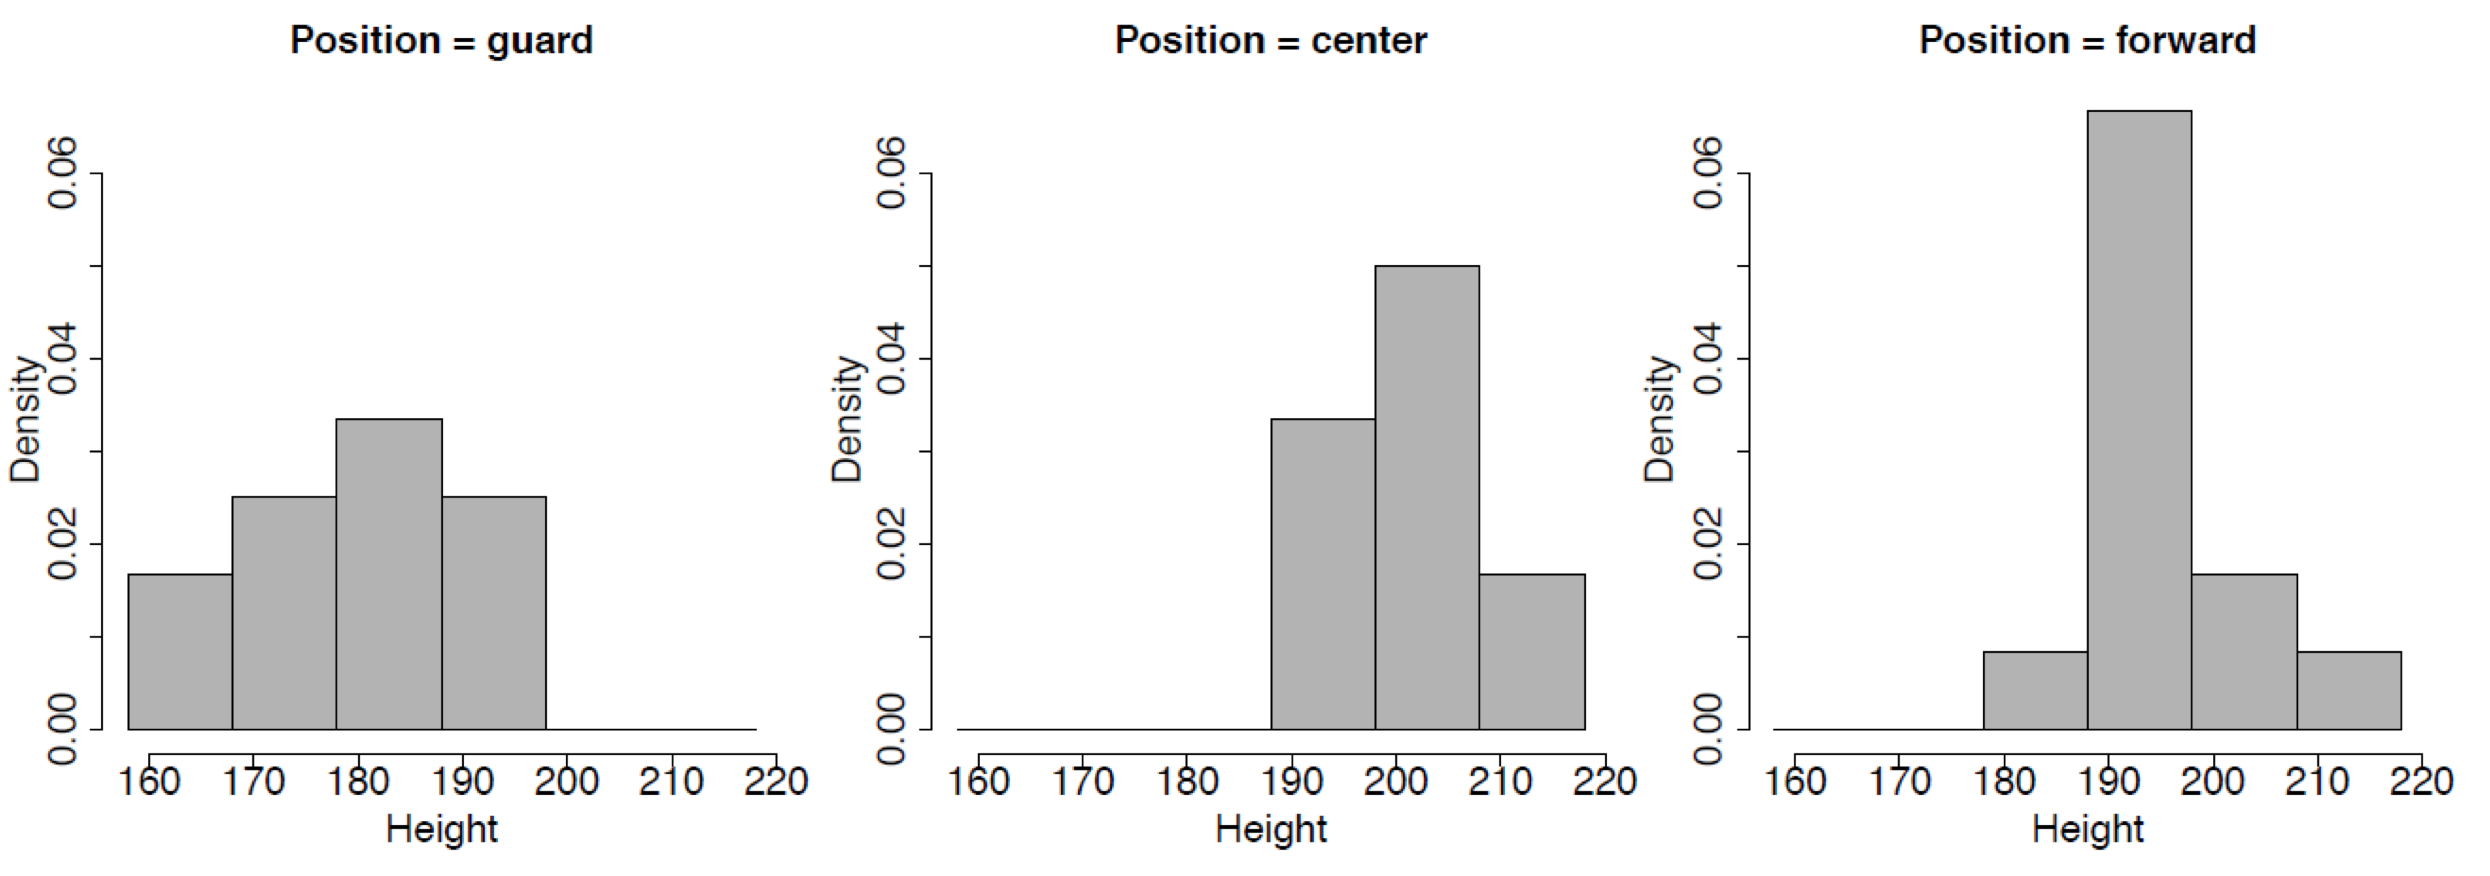
\includegraphics[width=\textwidth]{assets/visualization_and_extraction/feature_relation/histo_strong.png}
    \subcaption{Height \textcolor{gray}{\footnotesize (6 bins)}: Relation to position}
  \end{subfigure}
  \caption{Collection of (conditioned) histograms \textcolor{gray}{\footnotesize (Conditioned on position)}}
  \label{fig:2_histoplot}
\end{figure}

Alternatively, \textbf{box plots} can be collected\sidenote{Collection of box plots} and utilized to identify relations. \begin{note}Figure \ref{fig:2_box_plot_coll} conducts the same relation between age or height to position. It further highlights the relatively strict separation of age for individual positions.\end{note}

\begin{figure}[H]
  \centering
  \begin{subfigure}{0.45\textwidth}
    \centering
    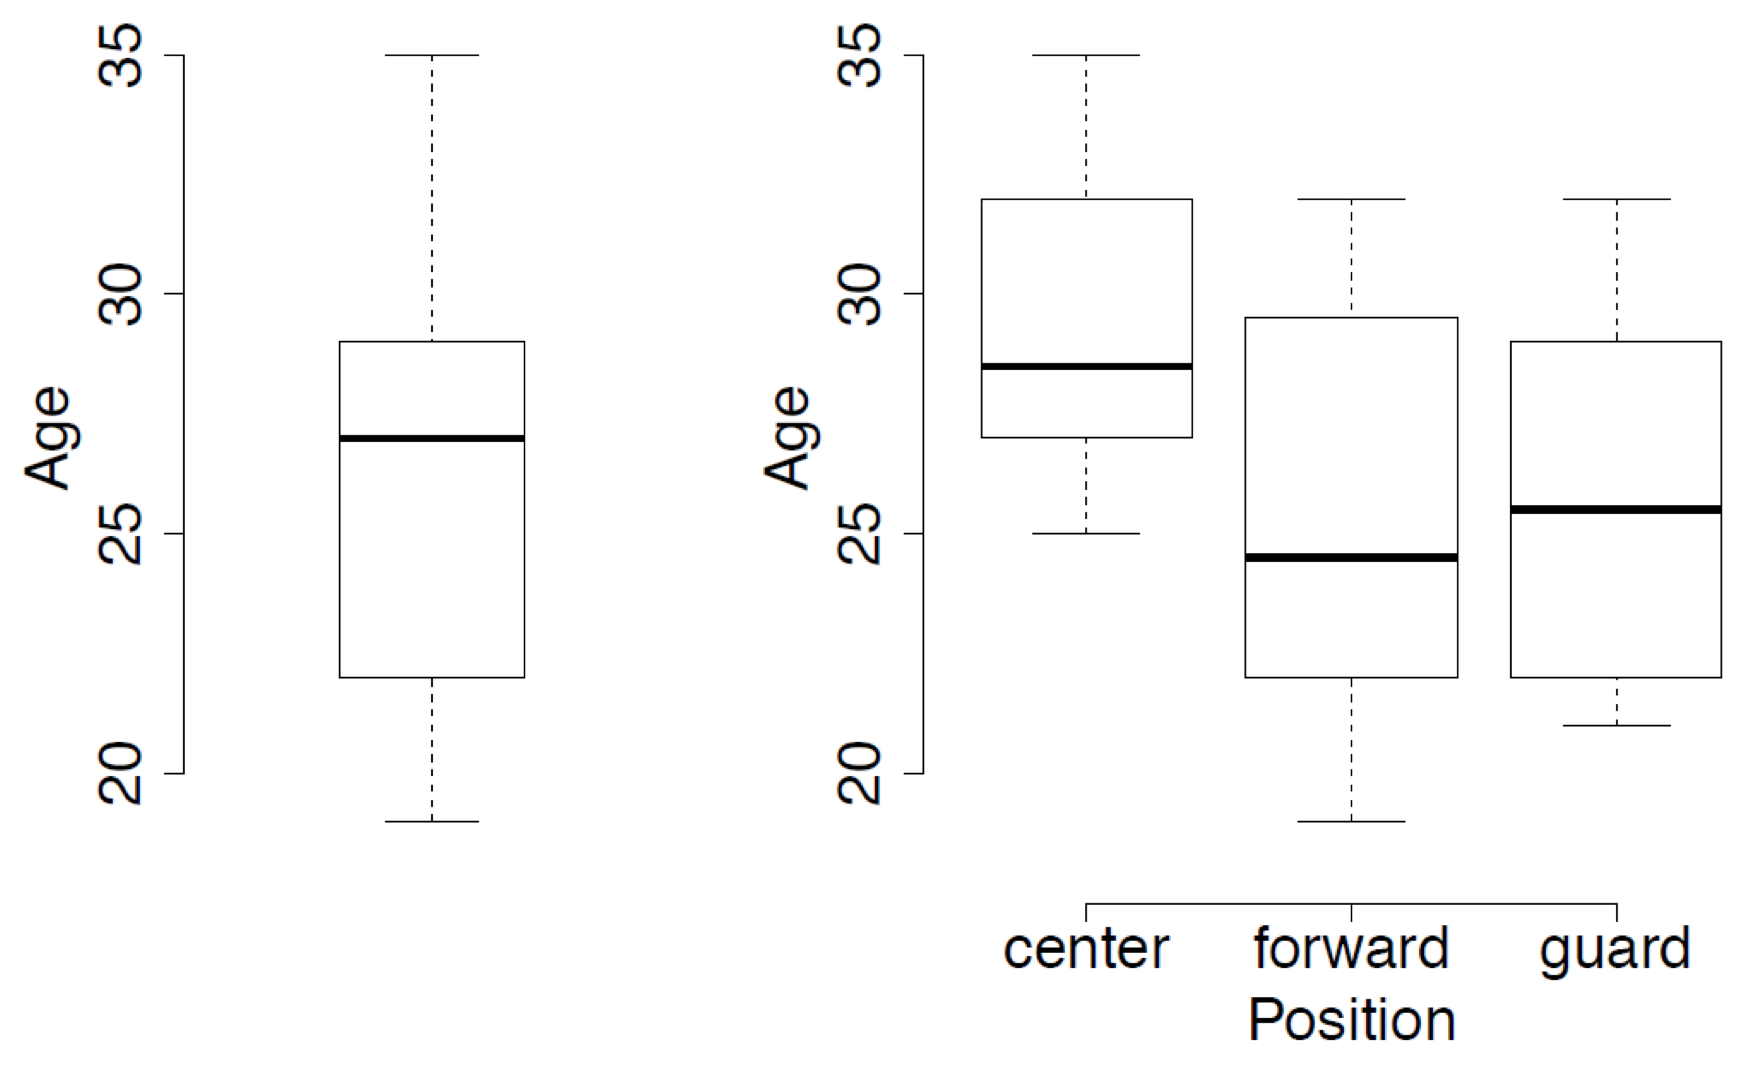
\includegraphics[width=\textwidth]{assets/visualization_and_extraction/feature_relation/box_weak.png}
    \subcaption{Age: Weaker relation to position}
  \end{subfigure}
  \hspace*{0.05\textwidth}
  \begin{subfigure}{0.45\textwidth}
    \centering
    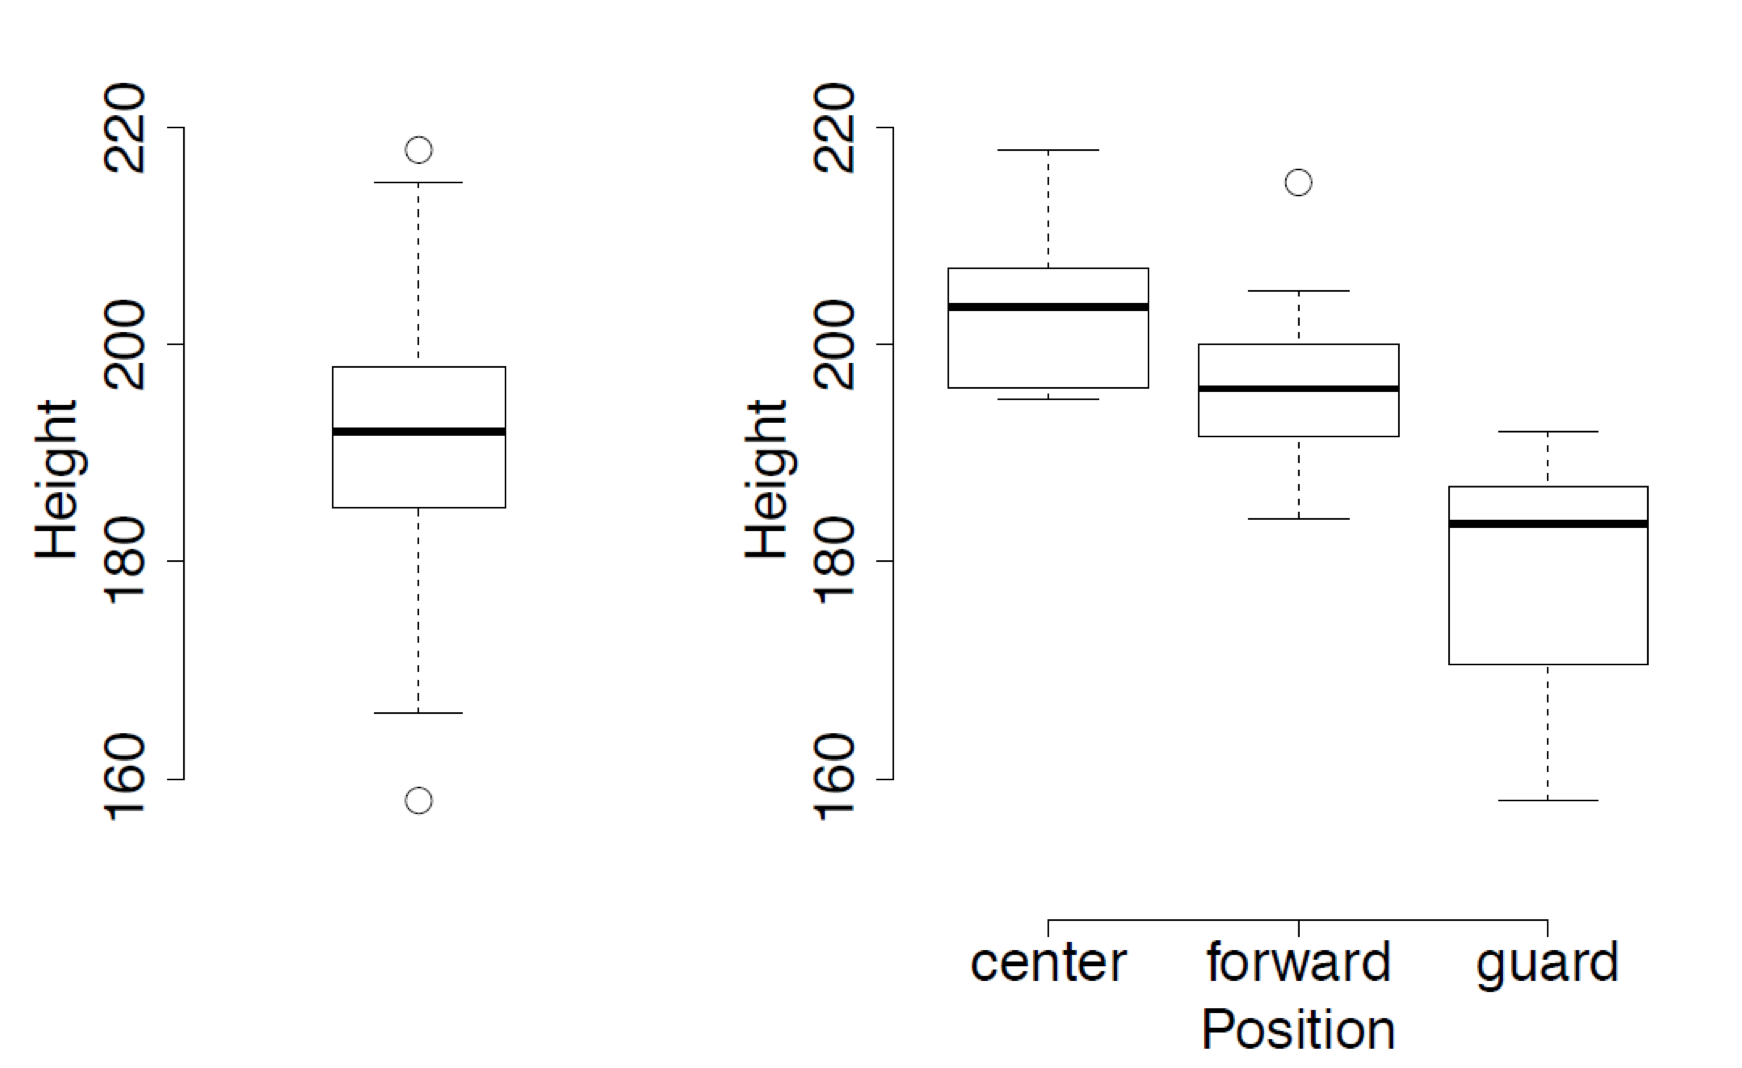
\includegraphics[width=\textwidth]{assets/visualization_and_extraction/feature_relation/box_strong.png}
    \subcaption{Height: Stronger relation to position}
  \end{subfigure}
  \caption{Collection of (conditioned) box plots \textcolor{gray}{\footnotesize (Conditioned on position)}}
  \label{fig:2_box_plot_coll}
\end{figure}

\subsubsection*{Descriptive statistics}

To not only see the relation but also classify it with values, we now introduce some basic descriptive statistics. Based on $n$ values $a_1, \dots, a_n$, we have the \textbf{sample mean} $\overline{a}$ and \textbf{sample variance} $var(a)$ and \textbf{standard deviation} $sd(a)$ as:
\begin{align*}
  \overline{a} = &\ \frac{1}{n}\sum_{i=1}^n a_i\sidenote{Sample mean}\allowdisplaybreaks\\
  var(a) = &\ \frac{\sum_{i=1}^n (a_i - \overline{a})^2}{n-1}\sidenote{Sample variance}\allowdisplaybreaks\\
  sd(a) = &\ \sqrt{var(a)} = \sqrt{\frac{\sum_{i=1}^n (a_i - \overline{a})^2}{n-1}}\sidenote{Standard deviation}
\end{align*}

A quick note on why we divide by $n-1$ and not $n$ for the calculation of $var(a)$. This is due to the estimated mean $\overline{a}$ instead of actual or true one $\hat{a}$. Simply put, since we can only estimate, we would rather overestimate the variance \begin{note}(divide by a smaller number)\end{note} instead of underestimating \begin{note}(divide by a larger number)\end{note} it. We would call a variance calculated by dividing by $n$ a biased estimator.

To classify the relation between features, based on $n$ pairs of values $(a_1, b_1), \dots, (a_n, b_n)$ we have the \textbf{sample covariance} $cov(a, b)$ and the \textbf{correlation} $corr(a, b)$ as: 
\begin{align*}
  cov(a, b) = &\ \frac{1}{n-1}\sum_{i=1}^n ((a_i - \overline{a})\times(b_i - \overline{b}))\sidenote{Sample covariance}\allowdisplaybreaks\\
  corr(a, b) = &\ \frac{cov(a, b)}{sd(a)\times sd(b)}\sidenote{Correlation}
\end{align*}

Covariance and correlation have the following properties:
\begin{align*}
  cov(a, b) \in &\ [-\infty, \infty] \text{ (unbounded)}\\
  cov(a, b) &\ \text{ is }\begin{array}{l}
    \text{positive } (+)\\\text{negative } (-)
  \end{array}\text{ if } a \text{ }\begin{array}{l}
    (\pm)\\(\pm)
  \end{array}\text{ and } b \text{ }\begin{array}{l}
    (\pm)\\(\mp)
  \end{array} \text{ are }\begin{array}{l}
    \text{the same}\\\text{different}
  \end{array}\allowdisplaybreaks\\\\
  corr(a, b) \in &\ [-1, 1] \text{ (normalized)}\\
  corr(a, b)&\ \begin{array}{l}
    >0\\<0\\=0
  \end{array}\text{ if } a \text{ and } b \text{ are }\begin{array}{l}
    \text{positively correlated}\\
    \text{negatively correlated}\\
    \text{independent}
  \end{array}
\end{align*}

\begin{figure}[H]
  \centering
  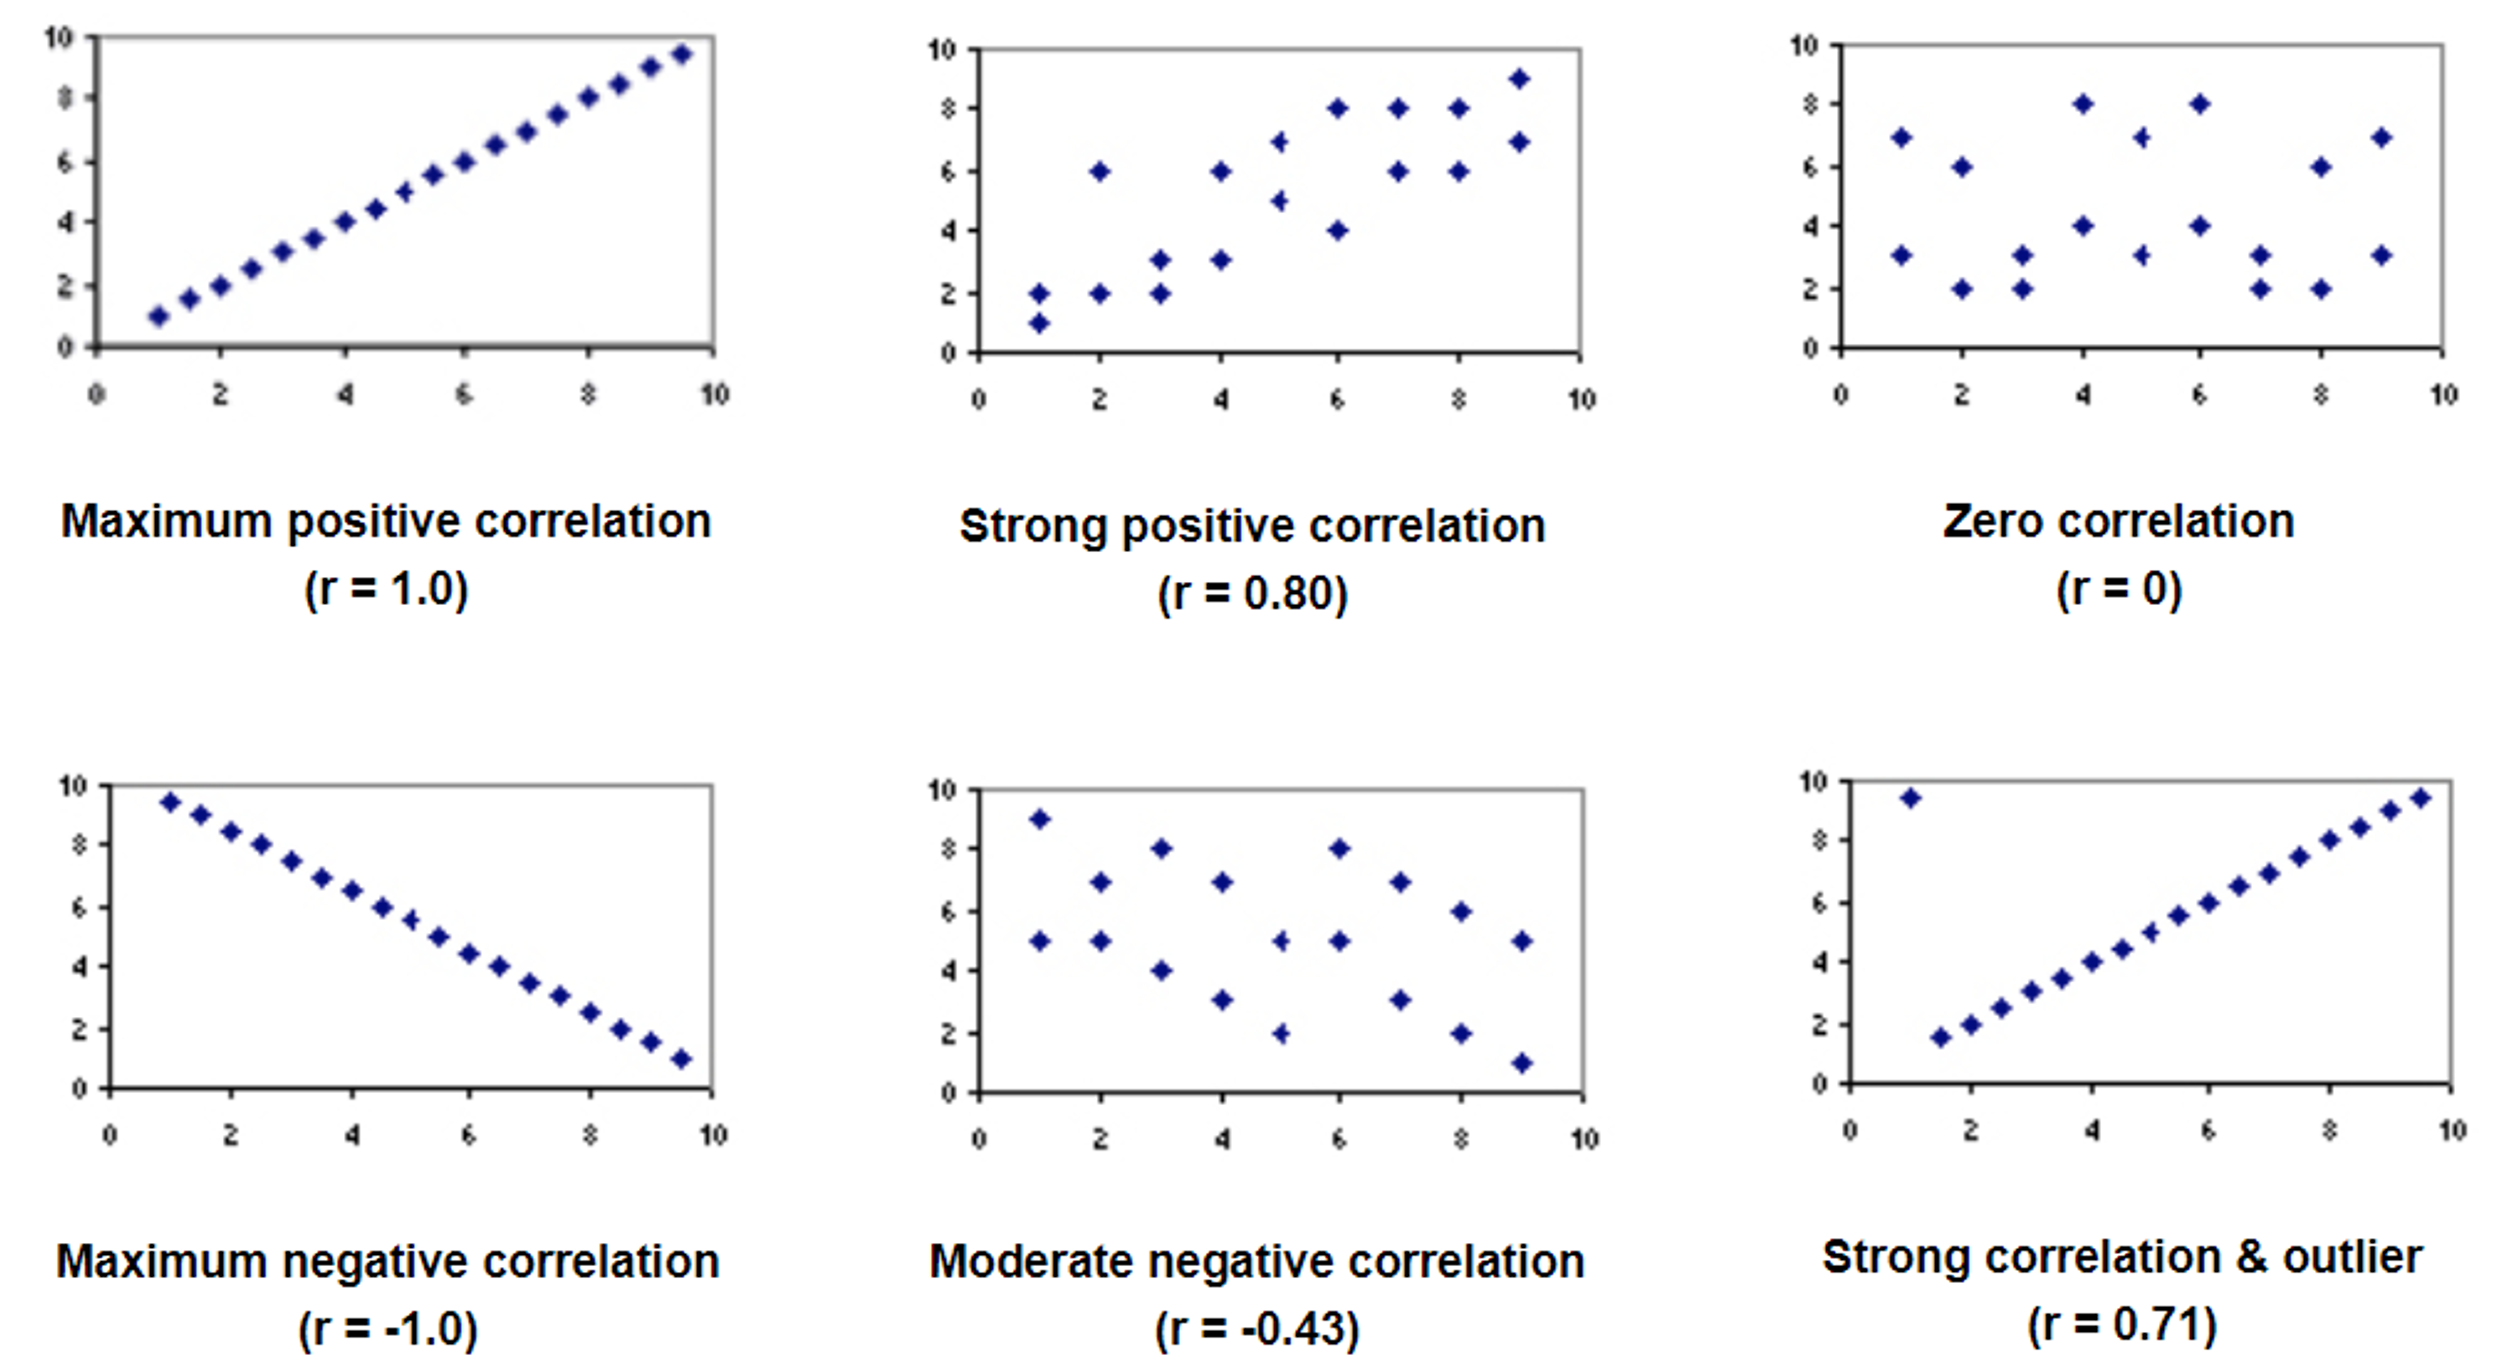
\includegraphics[width=\textwidth]{assets/visualization_and_extraction/feature_relation/corr_examples.png}
  \caption{Different correlation examples with scatter plot}
  \label{fig:2_corr_examples}
\end{figure}

With the new knowledge, we can expand our previous SPLOM diagram with the \textbf{correlation matrix} values. A correlation matrix looks as follows:
\begin{align*}
  \underset{\{a, b, \dots, z\}}{corr\text{\color{mathblue}  matrix}}\sidenote{Correlation matrix} = \left(\begin{array}{cccc}
    corr(a,a) & corr(a,b) & \cdots & corr(a,z)\\
    corr(b,a) & corr(b,b) & \cdots & corr(b,z)\\
    \vdots & \vdots & \ddots & \vdots\\
    corr(z,a) & corr(z,b) & \cdots & corr(z,z)
  \end{array}\right)
\end{align*}
with $corr(f_1, f_2) = corr(f_2, f_1)$ for all $f_1, f_2 \in \{a, b, \dots, z\}$ making the correlation matrix symmetric.

The updated SPLOM diagram, which basically contains the same information twice (just flipped) now also shows the correlation values as can be seen in \ref{fig:2_splom_corr}.
\begin{figure}[H]
  \centering
  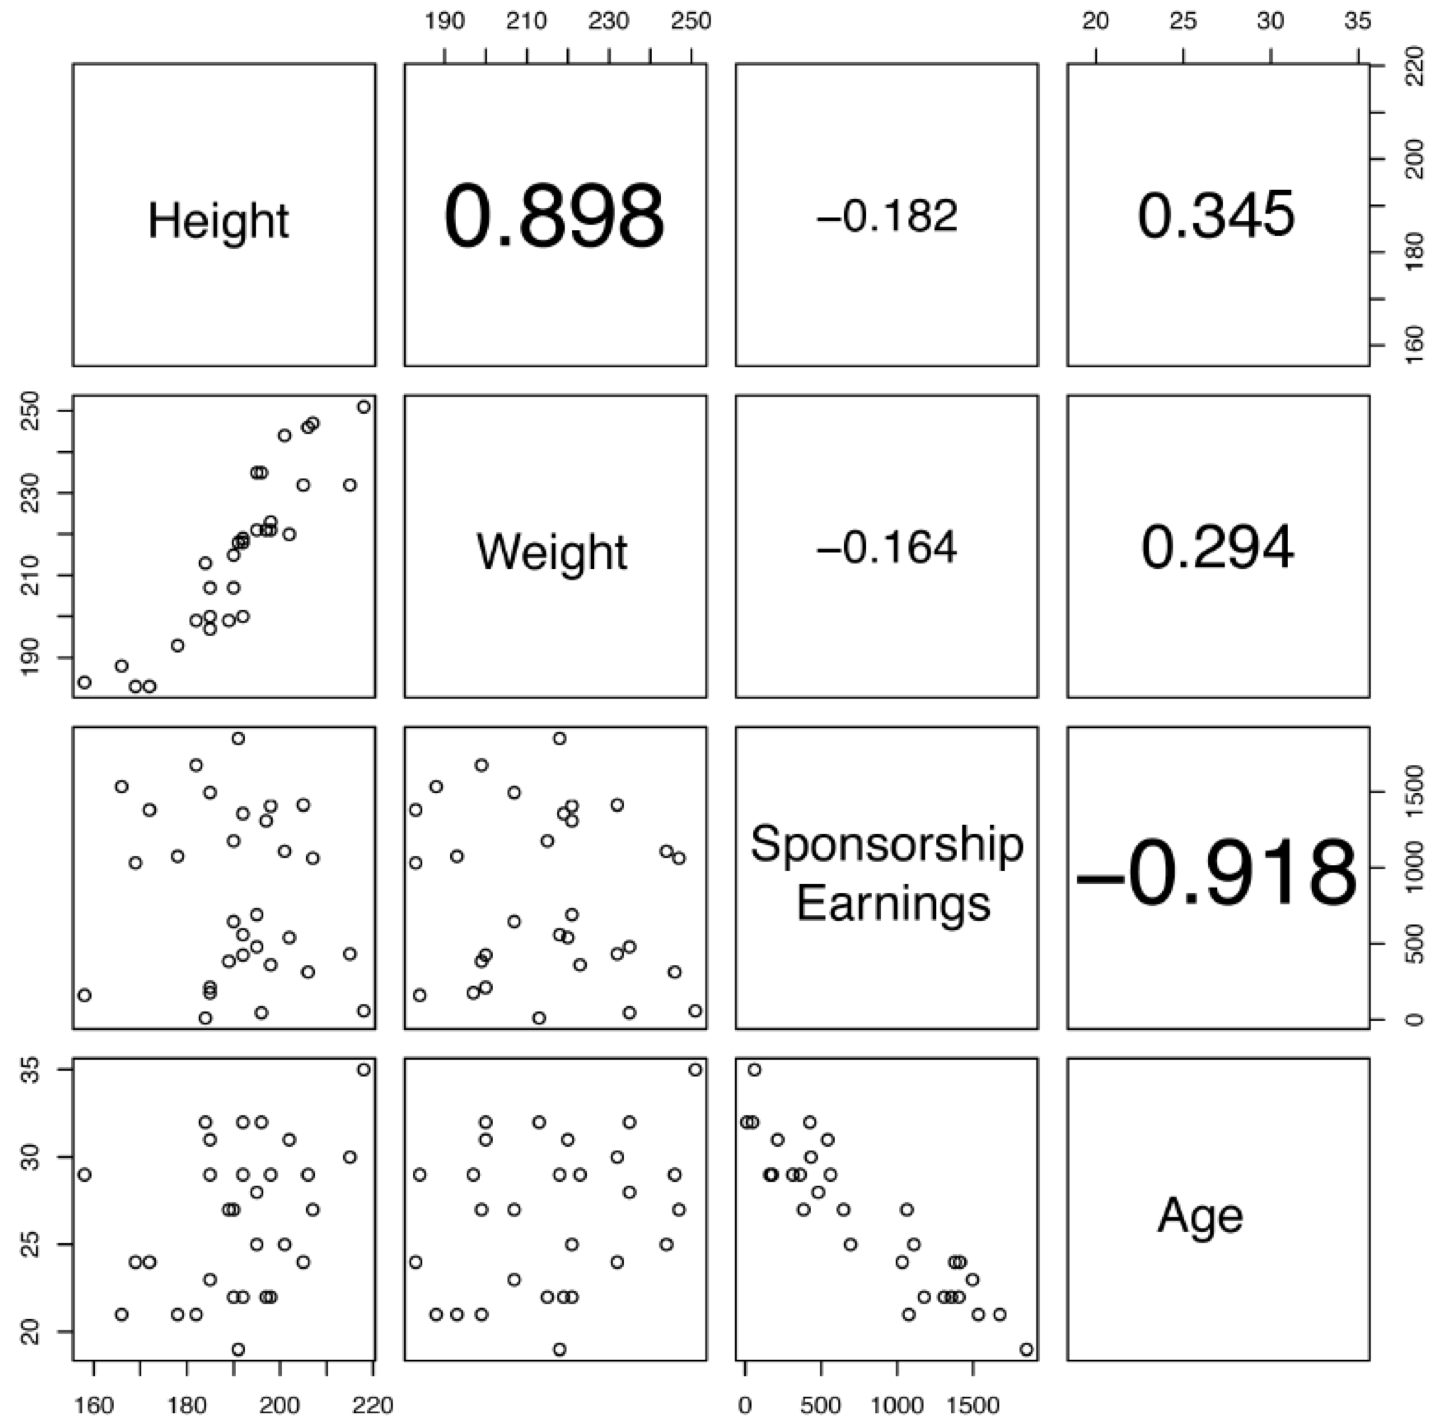
\includegraphics[width=0.6\textwidth]{assets/visualization_and_extraction/feature_relation/splom_updated.png}
  \caption{Scatter plot matrix of four features with according $corr$-values}
  \label{fig:2_splom_corr}
\end{figure}